% Results: decision latency (EXP-043). Numbers are macros from
% tables/generated/numbers.tex, computed by analysis/latency_outputs.py.
Table~\ref{tab:latency} reports per-call latency on one host for three implementations of each model: scikit-learn called with a one-row pandas DataFrame, which is how the model is called inside the experiment code; scikit-learn called with a NumPy array on one thread; and ONNX Runtime on one thread, used only where the exported model reproduced scikit-learn's decisions (\LatOnnxOK{} of \LatOnnxN{} exports, with decision agreement of at least \LatOnnxAgreeMin). A no-op call has a 99th percentile of \LatFloorPnn{}\,ms, so the platform floor does not affect the comparisons.

The implementation moves latency more than the architecture does (Fig.~\ref{fig:latency}). For LR, the DataFrame path costs \LatLRdfPfifty{}\,ms at the median against \LatLRarrPfifty{}\,ms for an array, the difference being input validation. RF predicting one row through its default thread pool takes \LatRFthreadsPfifty{}\,ms at the median, \LatRFarrPfifty{}\,ms on one thread and \LatRFonnxPfifty{}\,ms in ONNX Runtime. Across architectures, the 99th percentile of ONNX Runtime lies between \LatOnnxPnnMin{} and \LatOnnxPnnMax{}\,ms on the radio layer, against up to \LatArrPnnMax{}\,ms for scikit-learn with arrays. A ranking of architectures by latency is really a ranking of implementations, and a comparison with measurements taken on other hosts or in other languages~\cite{obiuwevwi2026realtime} says nothing about the architectures. For context only, Obiuwevwi et al. measure inference inside an OpenAirInterface and FlexRIC near-real-time RIC in the microsecond range for logistic regression and a small MLP~\cite{obiuwevwi2026realtime}, within an order of magnitude of our ONNX Runtime figures.

For a window-level detector the decision path is window aggregation followed by inference. Aggregating one 16-record window costs \LatAggPnn{}\,ms at the 99th percentile, and the upper bound of the 99th percentile of aggregation plus ONNX inference is at most \LatEtoEPnnHiMax{}\,ms across the architectures with a verified export. On this host that path would meet any budget in the specified range. A repeat of the radio measurement on the same host, which kept every call for Fig.~\ref{fig:latency}, gave medians \LatRepMedRatioMin{} to \LatRepMedRatioMax{} times those of Table~\ref{tab:latency} (median ratio \LatRepMedRatio), so per-call latency on a host without CPU isolation depends on the state of the host as well as on the model; the upper 95\% bound of the 99th percentile of aggregation plus ONNX inference was still at most \LatRepEtoEPnnHiMax\,ms. Whether a deployment does is decided by the terms we did not measure: indication decoding, control encoding, and queueing inside a RIC.

For a flow-level detector, features cost more than inference. On the three DDoS captures of \DA{}, the vectorized exporter produces flow records at \LatExtrMin{} to \LatExtrMax{}\,ms per flow, \LatExtrSpeedMin{} to \LatExtrSpeedMax{} times faster than the per-packet reference implementation on the same captures (\LatExtrRefMin{} to \LatExtrRefMax{}\,ms per flow); per-flow cost grows with packets per flow. On the \LatEqCaptures{} captures compared record by record, the two exporters agree exactly in packets and bytes on all \LatEqKeys{} shared IPv4 flow keys; the reference additionally emits \LatRefOnlyMin{} and \LatRefOnlyMax{} IPv6 link-local keys, which the vectorized exporter, being IPv4-only, does not parse. Mapping one exported record onto the shared space through the pandas code of our pipeline costs a further \LatMapPfifty{}\,ms at the median, while ONNX inference on flow features costs at most \LatNetOnnxPnnMax{}\,ms at the 99th percentile. These figures describe a Python pipeline on one host: they locate the cost in feature construction, and say nothing about what a native exporter at the user plane would cost.

\begin{table*}[t]
\caption{Per-call latency in milliseconds on one host (Section~\ref{sec:setup}): 20,000 calls after 1,000 warm-up calls, one thread per library, garbage collection enabled. Emulated: no RIC in the path. Radio path $\overline{p}_{99}$: upper 95\% bound of the 99th percentile of window aggregation plus ONNX inference. Dashes: no export that reproduced scikit-learn's decisions.}
\label{tab:latency}
\centering
\footnotesize
% GENERATED by analysis/make_tables.py on 2026-09-25
% source: EXP-043 latency_stages
% commit: a5e2ab8
% DO NOT EDIT. Edit the generator, then re-run `make tables`.
\begin{tabular}{lccccccccc}
\toprule
& \multicolumn{2}{c}{sklearn, DataFrame} & \multicolumn{2}{c}{sklearn, array} & \multicolumn{2}{c}{ONNX Runtime} & Radio path & \multicolumn{2}{c}{Flow layer, $p_{99}$} \\
Model & $p_{50}$ & $p_{99}$ & $p_{50}$ & $p_{99}$ & $p_{50}$ & $p_{99}$ & $\overline{p}_{99}$ & array & ONNX \\
\midrule
LR & 0.44 & 0.72 & 0.11 & 0.17 & 0.010 & 0.023 & 0.12 & 0.16 & 0.025 \\
DT & 0.31 & 0.52 & 0.03 & 0.04 & 0.010 & 0.014 & 0.11 & 0.06 & 0.024 \\
RF & 6.25 & 12.99 & 5.57 & 21.50 & 0.012 & 0.024 & 0.10 & 4.45 & 0.029 \\
XGB & 0.73 & 1.00 & 0.16 & 0.32 & 0.011 & 0.021 & 0.09 & 0.40 & 0.024 \\
HGB & 1.48 & 2.72 & 1.17 & 1.92 & 0.013 & 0.035 & 0.12 & 1.22 & 0.034 \\
MLP & 0.43 & 0.67 & 0.11 & 0.21 & 0.017 & 0.035 & 0.11 & 0.15 & 0.037 \\
\bottomrule
\end{tabular}

\end{table*}

\begin{figure}[t]
\centering
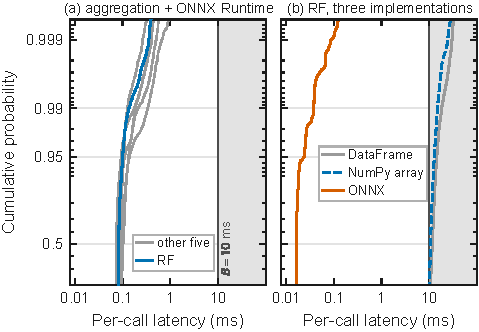
\includegraphics[width=\columnwidth]{../figures/generated/fig_rev_latency.pdf}
\caption{Empirical distribution of per-call latency for the radio layer on one host, 20,000 calls per stage, on a logit scale so that the median, 95th and 99th percentiles are all visible. (a) The decision path of the deployability test, window aggregation followed by ONNX Runtime, for the six architectures. (b) One architecture, RF, under the three implementations of Table~\ref{tab:latency}. The shaded region lies beyond $B=10$\,ms, the smallest budget in the specified range. Only feature construction and inference are timed; indication decoding, control encoding, and queueing, which need a RIC in the path, are not. The curves come from a repeat of the measurement that kept every call (EXP-060); Table~\ref{tab:latency} reports the original run.}
\label{fig:latency}
\end{figure}
